\chapter{ПРОГРАММНАЯ РЕАЛИЗАЦИЯ}
\section{Используемые программные средства}

В данной работе было использованы следующие языки программирования:
\begin{itemize}
    \item Python
    \item Golang
\end{itemize}

Изначально все математические модели были реализованы на языке Python с использованием библиотеки numpy, это было сделано для проверки их работоспособности. Несомненным приемуществом работы Python является его простота в использовании, а так же большое количество готовых библиотек, сильно 
упрощающих разработку. Но так же Python является языком динамической типизации, что значительно влияет на скорость его работы, поэтому для задач,
требующих больших вычислительных мощностей, которой как раз и является данная задача, использование Python является нецелесообразным. Поэтому дальнейшая
разработка производилась на языке Golang.

\subsection*{Язык Golang}

Среди современных языков программирования следует выделить язык программирования Go, реализация которого была выполнена командой разработчиков фирмы Google \cite{GoTour}. Язык Go разрабатывался как язык программирования для создания высокоэффективных программ, работающих на современных распределённых системах и многоядерных процессорах. Он может рассматриваться как попытка создать замену языкам Си и C++. 

Основные возможности Golang:
\begin{itemize}
    \item Go — язык со строгой статической типизацией. Доступен автоматический вывод типов, для пользовательских типов — "утиная типизация".
    \item Полноценная поддержка указателей, но без возможности применять к ним арифметические операции, в отличие от C/C++/D.
    \item Использование динамических массивов, хеш-таблиц, срезов (слайсов), вариант цикла для обхода коллекции.
    \item Средства функционального программирования: неименованные функции, замыкания, передача функций в параметрах и возврат функциональных значений.
    \item Автоматическое управление памятью со сборщиком мусора.
    \item Средства объектно-ориентированного программирования, но без поддержки наследования реализации (наследуются только интерфейсы). По большому счёту, Go является процедурным языком с поддержкой интерфейсов.
    \item Средства параллельного программирования: встроенные в язык потоки (go routines), взаимодействие потоков через каналы и другие средства организации многопоточных программ.
    \item Достаточно лаконичный и простой синтаксис, основанный на Си.
\end{itemize}

Go содержит конструкцию, которая позволяет запустить исполнение вызова некоторой функции в отдельном потоке. Такая функция называется в Go горутиной (англ. goroutine), ниже приведен пример оператора вызова горутины: 

\begin{lstlisting}[numbers=none, language=Golang, caption=Пример вызова горутины]
    go f(args) 
\end{lstlisting} 

Каналы используются в качестве средства взаимодействия между горутинами. Помимо каналов в пакете \textit{sync} содержатся такие примитивы синхронизации, как мьютексы или условные переменные, однако их рекомендуется применять только для низкоуровневых библиотек.

Каналы в Go типизированы и являются объектами первого класса. Их можно посылать в функции, возвращать из функций, присваивать переменным и полям структур, а также пересылать по каналам. Они могут работать только в одну сторону или в обе. Причем, если обычный двунаправленный канал передать в функцию, где он используется, например, только на прием, его можно промаркировать соответствующим образом в списке параметров функции и компилятор проверит правильность его использования. Обычные каналы блокируют горутину, которая пытается получить из или послать что-то в канал, пока с другой стороны не будет произведено соответсвующее обратное действие. Но канал может иметь буфер, который может накапливать и отдавать накопленное определенное количество значений без блокировки. Канал может быть закрыт встроенной функцией \textit{close}, после этого посылка в него значений приведет к "панике", так в данном языке называется экстренное завершение программы в случае ошибки. Если закрытый канал имеет непустой буфер, эти значения все еще могут быть получены. Но когда буфер уже пуст или его нет, закрытый канал при попытке чтения будет выдавать нулевые значения того типа, для пересылки которых он создан. То есть, закрытый строковый канал будет выдавать пустые строки, целочисленный — нули, канал указателей — nil. Более подробно горутины и в целом язык Golang описывается в книге \cite{ProgrammingInGo}

Также неоспоримым приемуществом Golang является его скорость работы и компиляции, сопоставимая с такими языками, как Java, C, C++. На рисунке \ref{fig:govs} сопоставлены популярные языки и Go, на примере часто встречающихся задач.

\begin{figure}[h]
    \centering
    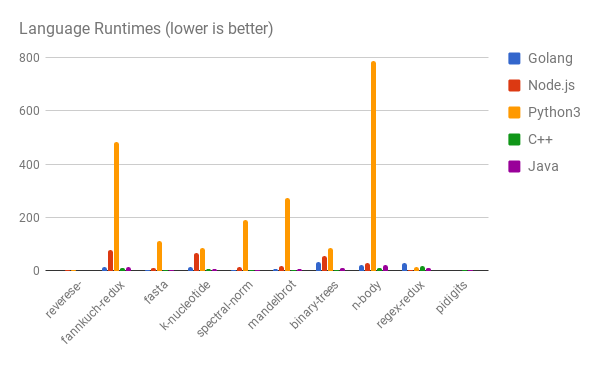
\includegraphics[width=0.9\textwidth]{golang-language-runtimes-1.png}
    \caption{Сопоставление Golang, Python, C++, Java, Node.js.}
    \label{fig:govs}
\end{figure}

Учитывая наличие сборщика мусора, времени компиляции сопоставимым с C++, а так же простотой синтаксиса и читабельностью кода, было решено остановиться на данном языке как на основном языке разработки. Так же в Golang есть возможноть исполнения кода, написанного на языке C, что позволяет уменьшить время работы программ, а так же использовать математические библиотке blas и lapack, которые реализованы в пакете \textbf{gonum}\cite{GoNum}. 